\begin{figure}[htbp]
\centering
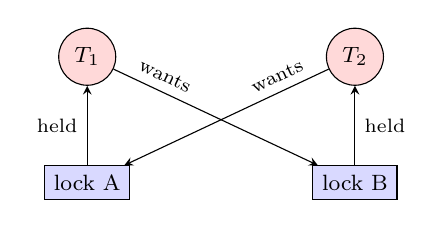
\begin{tikzpicture}[font=\footnotesize, >=stealth, x=1cm, y=1cm]
  \node[draw, circle, fill=red!15] (t1) at (0,1.6) {$T_1$};
  \node[draw, circle, fill=red!15] (t2) at (3.4,1.6) {$T_2$};
  \node[draw, rectangle, fill=blue!15] (la) at (0,0) {lock A};
  \node[draw, rectangle, fill=blue!15] (lb) at (3.4,0) {lock B};
  \draw[->] (t1) -- (lb) node[pos=0.22,above,sloped]{\scriptsize wants};
  \draw[->] (t2) -- (la) node[pos=0.22,above,sloped]{\scriptsize wants};
  \draw[->] (la) -- (t1) node[midway,left]{\scriptsize held};
  \draw[->] (lb) -- (t2) node[midway,right]{\scriptsize held};
\end{tikzpicture}
\caption{The wait-for graph of a textbook deadlock: $T_1$ holds A,
wants B; $T_2$ holds B, wants A. A cycle in this graph is a
deadlock --- and a global lock \emph{order} is what prevents cycles
from ever forming.}
\label{fig:deadlock13}
\end{figure}
